%% =====================================================================
%% Technical Report -- Data Engineering (CO5173), HCMUT -- Group 27
%% Kimball Dimensional Data Warehouse for Banking Cash-Flow Analytics (Berka)
%%
%% Format and structure follow the IEEE technical report template in
%% LaTeX_Template_for_Technical_Report/ (IEEEtran v1.8, peerreview).
%% IEEEtran.cls must sit next to this file.
%% Build: tectonic main.tex, or pdfLaTeX / XeLaTeX on Overleaf (run twice)
%% Items in red [TODO] are pending decisions of the group.
%% =====================================================================

\documentclass[peerreview]{IEEEtran}
\usepackage{cite}      % Tidies up citation numbers.
\usepackage{url}       % Provides better formatting of URLs.
\usepackage{iftex}
\ifPDFTeX
  \usepackage[utf8]{inputenc}
\fi
\usepackage{booktabs}  % \toprule, \midrule and \bottomrule in tables
\usepackage{graphicx}
\graphicspath{{figures/}}

% ---------- Additional packages ----------
\usepackage{amsmath,amssymb}
\usepackage{array}
\usepackage{xcolor}
\usepackage{listings}
\usepackage{tikz}
\usetikzlibrary{arrows.meta,positioning,fit}
\usepackage[hidelinks]{hyperref}

% ---------- Float placement ----------
\setcounter{topnumber}{3}
\setcounter{bottomnumber}{2}
\setcounter{totalnumber}{5}
\setcounter{dbltopnumber}{2}
\renewcommand{\topfraction}{0.85}
\renewcommand{\bottomfraction}{0.6}
\renewcommand{\textfraction}{0.1}
\renewcommand{\floatpagefraction}{0.85}
\renewcommand{\dbltopfraction}{0.85}
\renewcommand{\dblfloatpagefraction}{0.85}

\hyphenation{op-tical net-works semi-conduc-tor}

% ---------- Helpers ----------
\newcommand{\todo}[1]{\textcolor{red}{[TODO: #1]}}
\newcommand{\tbl}[1]{\texttt{#1}}
\newcolumntype{L}[1]{>{\raggedright\arraybackslash}p{#1}}

\lstdefinestyle{code}{
  basicstyle=\ttfamily\scriptsize,
  keywordstyle=\color{blue!70!black}\bfseries,
  commentstyle=\color{green!40!black}\itshape,
  stringstyle=\color{orange!70!black},
  breaklines=true,
  frame=single,
  framesep=3pt,
  columns=fullflexible,
  keepspaces=true,
  showstringspaces=false,
  captionpos=b
}
\lstset{style=code}


\begin{document}

% paper title
\title{A Kimball Dimensional Data Warehouse for Banking Cash-Flow Analytics: \\
Design, Implementation, and Evaluation \\ with Spark, ClickHouse, and PostgreSQL}

% author names and affiliations
\author{Kiet Ho Tuan Nguyen, Quan Minh Tran, Van Ngoc Huynh, Hai Ngoc Ho \\
Group 27 --- Data Engineering (CO5173), Semester 1, 2026--2027\\
Faculty of Computer Science and Engineering\\
Ho Chi Minh City University of Technology (HCMUT), VNU-HCM\\
Instructor: Assoc. Prof. Dr. Chau Thi Ngoc Vo\\
}
\date{\todo{submission date}}

% make the title area
\maketitle
\tableofcontents
\listoffigures
\listoftables

\IEEEpeerreviewmaketitle

\begin{abstract}
A bank needs trusted answers on how money flows, what happened on an account, and whether
the data behind those answers can be trusted. We build and evaluate a data engineering
solution for these needs on the Berka dataset of a Czech bank (1,056,320 transactions,
1993--1998), extended with a simulated membership tier whose history must be preserved. The
solution is a Kimball data warehouse---one transaction fact and five dimensions, including a
Type~2 customer dimension---loaded in batches by Apache Spark through a Parquet data lake into
ClickHouse, with a PostgreSQL operational store for runs, rejected records, fraud alerts, and
backups, and one Streamlit application serving three user groups and eight business
requirements. Eight evaluation scenarios, each reconciled with the source, pass all 38
checks, and cash-flow totals match the source to the cent. Four benchmarks, each changing one
factor, show that ClickHouse answers aggregation queries 3.3--22 times faster than the same
star schema in PostgreSQL (7--28 times on a ten-fold copy) in 8.7 times less space; that a
One Big Table saves only milliseconds but must rewrite 150,058 rows to correct one district;
and that the operational store is 8--70 times faster in PostgreSQL, which also enforces
integrity rules that ClickHouse does not. Every requirement is answered in one to three
interactions.
\end{abstract}


%% =====================================================================
\section{Introduction}
\label{sec:intro}

Every deposit, payment, and withdrawal of a bank leaves a record. Aggregated, these records
show how money flows through the bank and how each account behaves---but raw transaction logs
cannot answer such questions directly: their codes are terse and partly missing, customer
attributes change without keeping their history, and nothing in them tells a user whether the
latest load succeeded or whether an earlier report still holds.

This report presents the project of Group~27 for the Data Engineering course (CO5173). The
application domain is \textbf{banking} and the solution is a \textbf{Kimball dimensional data
warehouse} \cite{kimball2013}. The objective is to show, with measurable evidence, that the
solution turns raw bank transactions into data that is correct, fast to query, and useful to
the bank's users. The main contributions are:
\begin{itemize}
  \item a star schema with a Type~2 customer dimension that keeps the history of a
        membership tier;
  \item a batch pipeline that isolates defective records, re-runs without duplicates, and
        records every run in an operational store, controlled from one application;
  \item an evaluation through eight scenarios reconciled with the source and four
        benchmarks against alternative solutions.
\end{itemize}
Section~\ref{sec:problem} defines the problem, Section~\ref{sec:solutions} the solutions,
Section~\ref{sec:criteria} the assessment criteria, Section~\ref{sec:method} the methodology,
Section~\ref{sec:analysis} the results, and Section~\ref{sec:conclusion} concludes.


%% =====================================================================
\section{Problem Definition}
\label{sec:problem}

\subsection{Problem Statement}
\begin{quote}
\emph{How can a bank's transaction data be engineered into a correct, performant, and
exploitable data warehouse whose loads are controlled, whose history is preserved, and which
demonstrably supports the business requirements of several user groups?}
\end{quote}

\subsection{User Groups and Business Requirements}
Three user groups were defined, each served by one tab of the application
(Table~\ref{tab:usergroups}). With four members, the course requires at least eight business
requirements (BRs); each comes with an evaluation scenario (KB01--KB08) whose expected result
is written before the data is loaded (Table~\ref{tab:brs}). Together they serve four
objectives: monitoring cash flow (BR01, BR08), serving account inquiries (BR02), reducing
fraud losses (BR03, BR04), and keeping data and operations trustworthy (BR05--BR07).

\begin{table}[!t]
\centering
\caption{User Groups}
\label{tab:usergroups}
\footnotesize
\setlength{\tabcolsep}{4pt}
\begin{tabular}{L{1.9cm} L{3.4cm} L{2.4cm}}
\toprule
\textbf{User group} & \textbf{Need} & \textbf{Tab / BRs} \\
\midrule
U01 Business manager & Cash-flow overview and history by tier & Overview / BR01 \\
U02 Analyst & Look up accounts; review and handle alerts & Analysis / BR02--BR04 \\
U03 Data engineer & Data quality, pipeline, backup, history & Operations / BR05--BR08 \\
\bottomrule
\end{tabular}
\end{table}

\begin{table*}[!t]
\centering
\caption{Business Requirements and Evaluation Scenarios}
\label{tab:brs}
\small
\begin{tabular}{l l L{6.6cm} L{6.4cm}}
\toprule
\textbf{ID} & \textbf{User} & \textbf{Business requirement} & \textbf{Evaluation scenario (expected result)} \\
\midrule
BR01 & U01 & Cash-flow overview: inflow, outflow, net flow, and count for a period, by tier, as daily or monthly charts & KB01: figures equal a query on the source \\
BR02 & U02 & Account activity: transactions and totals of an account over a period & KB02: transactions equal the source, one by one \\
BR03 & U02 & Fraud detection: after each load, alerts with a reason and evidence & KB03: a prepared fraud batch raises the expected alerts \\
BR04 & U02 & Alert handling: \emph{new / in review / resolved}, with notes and history & KB04: status changes recorded and visible in the UI \\
BR05 & U03 & Data control: validate each batch, isolate failing records with reasons & KB05: a batch with deliberate errors is split correctly \\
BR06 & U03 & Pipeline monitoring: steps, status, times, counts, cause of failure & KB06: a failed step and its cause are identified \\
BR07 & U03 & Backup and restore of the six warehouse tables, SCD history included & KB07: after a restore, the figures equal the backup \\
BR08 & U03 & History report: a tier change must not alter reports of earlier periods (SCD2) & KB08: old period unchanged, new period by the new tier \\
\bottomrule
\end{tabular}
\end{table*}

\subsection{Data Source}
\label{sec:data-source}
The Berka dataset \cite{berka1999} holds the anonymized records of a Czech bank. Each Berka
file stands in for a bank system (Table~\ref{tab:sources}); loans, standing orders, and cards
are outside the BRs. The 1,056,320 transactions grow from 28,205 in 1993 to 322,277 in 1998,
and each account has 9 to 675 transactions (median 208). Every account has exactly one owner,
and 409 accounts belong to a branch district other than the owner's residence, so the district
plays two roles. The \tbl{type} code gives the direction of money (Table~\ref{tab:types});
amounts are never negative. Profiling reproduced 14 of the 15 figures of the team's earlier
survey of the dataset.

\begin{table}[!t]
\centering
\caption{Source Files}
\label{tab:sources}
\footnotesize
\setlength{\tabcolsep}{4pt}
\begin{tabular}{L{2.5cm} L{3.2cm} r}
\toprule
\textbf{File} & \textbf{Stands in for} & \textbf{Rows} \\
\midrule
\tbl{trans} & Core banking system & 1,056,320 \\
\tbl{account} & Account registry & 4,500 \\
\tbl{client}, \tbl{disp} & Customer master (owners) & 5,369 \\
\tbl{district} & Reference data (77 districts) & 77 \\
\tbl{customer\_profile\_\allowbreak simulated} & Loyalty system (simulated tier) & 4,500 \\
\bottomrule
\end{tabular}
\end{table}

\begin{table}[!t]
\centering
\caption{Transaction Types and Cash-Flow Direction (Amounts in CZK)}
\label{tab:types}
\footnotesize
\setlength{\tabcolsep}{2.5pt}
\begin{tabular}{l l r r r r}
\toprule
\textbf{Type} & \textbf{Dir.} & \textbf{Count} & \textbf{Share} & \textbf{Median} & \textbf{Total (M)} \\
\midrule
VYDAJ (debit) & OUT & 634,571 & 60.07\% & 2,042 & 2,821.7 \\
PRIJEM (credit) & IN & 405,083 & 38.35\% & 1,600 & 3,227.5 \\
VYBER (withdrawal) & OUT & 16,666 & 1.58\% & 12,103 & 208.6 \\
\bottomrule
\end{tabular}
\end{table}

\subsection{Data Quality Defects}
\label{sec:data-quality}
The defects concern the classification of transactions, not the amounts
(Table~\ref{tab:dq}, by ISO/IEC 25012 \cite{iso25012}).

\begin{table*}[!t]
\centering
\caption{Data Quality Defects by ISO/IEC 25012 Characteristic}
\label{tab:dq}
\small
\begin{tabular}{L{2.3cm} L{7.0cm} L{5.4cm}}
\toprule
\textbf{Characteristic} & \textbf{Finding} & \textbf{Handling} \\
\midrule
Completeness & \tbl{operation} empty in 183,114 transactions; \tbl{k\_symbol} NULL in 481,881 and blank in 53,433 & Explicit member \texttt{NOT\_RECORDED}; no row dropped \\
Consistency & Two encodings of ``missing''; padded codes; 17 combinations that mean 15 & Standardized into a junk dimension of 15 profiles \\
Understand\-ability & Czech codes (e.g., \texttt{PRIJEM}, \texttt{SIPO}) & Readable names and a cash-flow direction \\
Accuracy & Birth date and gender packed into one ``birth number'' & Decoded into \tbl{gender} and \tbl{birth\_date} \\
Currentness & No attribute with a change history & Simulated membership tier with effective dates \\
\bottomrule
\end{tabular}
\end{table*}

\subsection{Simulated Membership Tier}
\label{sec:tier}
BR01 and BR08 need an attribute that changes over time. A deterministic script assigns each of
the 4,500 owners a tier by the inflow of the first year of the account: Standard (below
150,000~CZK, 2,075 owners), Silver (to 300,000, 1,438), Gold (to 550,000, 698), and Platinum
(289). A year-end re-evaluation of 1998, effective 1999-01-01, changes the tier of 618 owners;
together with their January 1999 transactions it forms scenario KB08.

\subsection{Scope}
\label{sec:other-directions}
Processing is in batches, not streaming. End-of-period balances, internal transfers, access
control, and the backup of the operational store are out of scope, and the solution runs on
one machine. Other uses of the data were considered and left out because they belong to other
business processes or user groups: loan default risk (\tbl{loan}), card analysis
(\tbl{card}, issuance only), recurring payments (\tbl{order}), customer segmentation, regional
economics (\tbl{district} attributes), and streaming fraud detection. The warehouse can be
extended with them later without changing the star schema.


%% =====================================================================
\section{Proposed Solutions}
\label{sec:solutions}

\subsection{First Solution: Kimball Star Schema on ClickHouse (Proposed)}
\label{sec:sol-kimball}

\subsubsection{Architecture}
The architecture has six blocks (Fig.~\ref{fig:arch}), drawn after the C4 model
\cite{c4model} and run with Docker Compose on one machine. \textbf{A} is the source.
\textbf{B}, the data lake, keeps an unchanged Parquet copy of every batch, so that any batch can
be traced and re-run. \textbf{C}, the PySpark pipeline, validates and standardizes a batch,
maintains the dimensions (SCD2 included), loads the fact, reconciles the batch with its input,
and evaluates the alert rules; every run and step is written to E. \textbf{D}, ClickHouse,
holds the star schema and a backup disk. \textbf{E}, PostgreSQL, holds what must be updated in
place and audited: runs, rejected records, alerts and their handling, and the backup catalog.
\textbf{F}, a Streamlit application with three tabs, reads D and E, writes alert handling to E,
and sends allow-listed commands to C.

\begin{figure*}[!t]
\centering
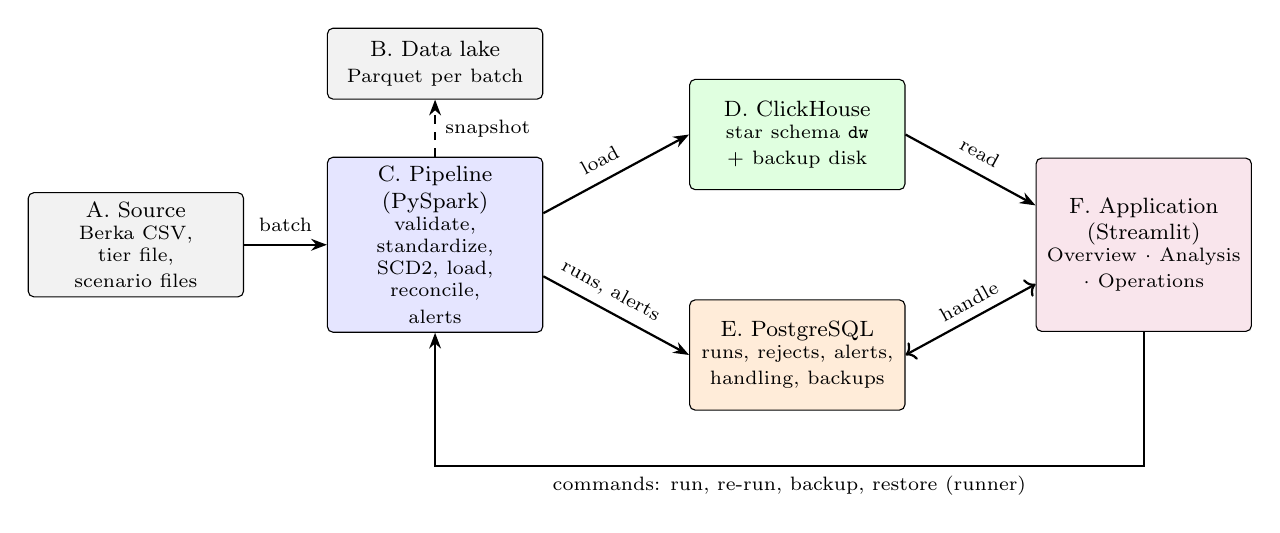
\begin{tikzpicture}[
  box/.style={draw, rounded corners=2pt, align=center, minimum height=1.1cm,
              text width=2.5cm, font=\footnotesize, fill=#1},
  box/.default=white,
  arr/.style={-{Stealth[length=2mm]}, thick},
  lbl/.style={font=\scriptsize, above=1pt}
]
\node[box=gray!10]                          (src)  at (0,0)      {A. Source\\{\scriptsize Berka CSV, tier file,\\scenario files}};
\node[box=gray!10, minimum height=0.9cm]    (lake) at (3.8,2.3)  {B. Data lake\\{\scriptsize Parquet per batch}};
\node[box=blue!10, minimum height=1.6cm]    (pipe) at (3.8,0)    {C. Pipeline (PySpark)\\{\scriptsize validate, standardize,\\SCD2, load, reconcile,\\alerts}};
\node[box=green!12, minimum height=1.4cm]   (dw)   at (8.4,1.4)  {D. ClickHouse\\{\scriptsize star schema \texttt{dw}\\+ backup disk}};
\node[box=orange!15, minimum height=1.4cm]  (ops)  at (8.4,-1.4) {E. PostgreSQL\\{\scriptsize runs, rejects, alerts,\\handling, backups}};
\node[box=purple!10, minimum height=2.2cm]  (app)  at (12.8,0)   {F. Application\\(Streamlit)\\{\scriptsize Overview $\cdot$ Analysis\\$\cdot$ Operations}};

\draw[arr] (src) -- node[lbl]{batch} (pipe);
\draw[arr, dashed] (pipe.north) -- node[right, font=\scriptsize]{snapshot} (lake.south);
\draw[arr] ([yshift=4mm]pipe.east) -- node[lbl, sloped, pos=0.45]{load} (dw.west);
\draw[arr] ([yshift=-4mm]pipe.east) -- node[above, sloped, font=\scriptsize, pos=0.4]{runs, alerts} (ops.west);
\draw[arr] (dw.east) -- node[lbl, sloped, pos=0.5]{read} ([yshift=5mm]app.west);
\draw[arr, <->] (ops.east) -- node[above, sloped, font=\scriptsize, pos=0.55]{handle} ([yshift=-5mm]app.west);
\draw[arr] (app.south) -- ++(0,-1.7) -| node[pos=0.25, below, font=\scriptsize]{commands: run, re-run, backup, restore (runner)} (pipe.south);
\end{tikzpicture}
\caption{Container-level architecture of the proposed solution (C4 model, level 2).}
\label{fig:arch}
\end{figure*}

\subsubsection{Dimensional Model}
Following Kimball's four steps \cite{kimball2013}, the business process is account
transactions and the grain is one fact row per transaction, so that reports and account
lookups use the same table (Fig.~\ref{fig:star}). \tbl{amount} is additive and is split into
inflow and outflow by the direction of the profile; \tbl{balance\_after} is semi-additive and
never summed. \tbl{dim\_customer} is \textbf{Type~2}: each tier is a version with its own
surrogate key and a validity interval [\tbl{valid\_from}, \tbl{valid\_to}), the current one
ending on 2299-12-31. \tbl{dim\_transaction\_profile} is a junk dimension of the 15 code
combinations, and \tbl{dim\_district} plays two roles through the account and the customer.
Each transaction is joined to the owner version valid on its date, with the date condition
inside the join: a tier change creates a version for future transactions without touching the
fact rows of earlier periods, and a transaction outside every version is rejected instead of
silently lost.

\begin{figure}[!htb]
\centering
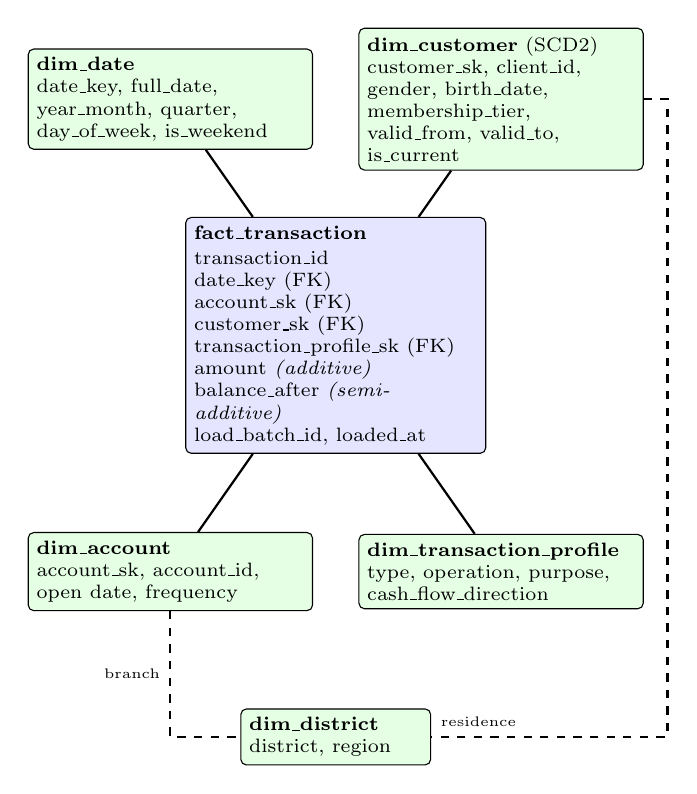
\begin{tikzpicture}[
  ent/.style={draw, rounded corners=2pt, align=left, font=\scriptsize,
              text width=3.4cm, inner sep=3pt},
  fact/.style={ent, fill=blue!10, text width=3.6cm},
  dim/.style={ent, fill=green!10},
  rel/.style={thick}
]
\node[fact] (f) at (0,0) {\textbf{fact\_transaction}\\[1pt]
transaction\_id\\ date\_key (FK)\\ account\_sk (FK)\\ customer\_sk (FK)\\
transaction\_profile\_sk (FK)\\ amount \emph{(additive)}\\
balance\_after \emph{(semi-additive)}\\ load\_batch\_id, loaded\_at};
\node[dim] (d) at (-2.1, 3.0) {\textbf{dim\_date}\\ date\_key, full\_date,\\ year\_month, quarter,\\ day\_of\_week, is\_weekend};
\node[dim] (c) at ( 2.1, 3.0) {\textbf{dim\_customer} (SCD2)\\ customer\_sk, client\_id,\\ gender, birth\_date,\\ membership\_tier,\\ valid\_from, valid\_to,\\ is\_current};
\node[dim] (a) at (-2.1,-3.0) {\textbf{dim\_account}\\ account\_sk, account\_id,\\ open date, frequency};
\node[dim] (t) at ( 2.1,-3.0) {\textbf{dim\_transaction\_profile}\\ type, operation, purpose,\\ cash\_flow\_direction};
\node[dim, text width=2.2cm] (g) at (0,-5.1) {\textbf{dim\_district}\\ district, region};
\draw[rel] (f) -- (d); \draw[rel] (f) -- (c);
\draw[rel] (f) -- (a); \draw[rel] (f) -- (t);
\draw[rel, dashed] (a.south) |- node[pos=0.25, left, font=\tiny]{branch} (g.west);
\draw[rel, dashed] (c.east) -- ++(0.3,0) |- node[pos=0.9, above, font=\tiny]{residence} (g.east);
\end{tikzpicture}
\caption{Star schema of the transaction business process; \tbl{dim\_district} plays two roles.}
\label{fig:star}
\end{figure}

\subsubsection{Pipeline}
The history is loaded as one reference batch and 72 monthly batches; each scenario is a
further batch. Each batch is validated with rules V1--V7 (Table~\ref{tab:vrules}); a failing
record is written with its rule, reason, and content to the operational store, and the rest of
the batch continues. Each batch is reconciled with its input (count and money). A re-run
skips transactions the batch has already loaded, and the fact table, a
\texttt{ReplacingMergeTree} keyed by transaction, cannot hold duplicates.

\begin{table}[!t]
\centering
\caption{Data Quality Rules Applied to Every Batch (BR05)}
\label{tab:vrules}
\footnotesize
\setlength{\tabcolsep}{4pt}
\begin{tabular}{l L{6.6cm}}
\toprule
\textbf{Rule} & \textbf{A record is rejected when} \\
\midrule
V1 & a mandatory field is missing \\
V2 & the account does not exist in the warehouse \\
V3 & the amount is negative or not a number \\
V4 & the date is invalid or outside the calendar \\
V5 & the type code is unknown \\
V6 & the transaction id is duplicated or loaded by another batch \\
V7 & no owner version is valid on the transaction date \\
\bottomrule
\end{tabular}
\end{table}

Fraud alerts (BR03) are computed after each load with two rules whose parameters are stored
in the operational store: \textbf{R1}, an account's outflow in a month exceeds three times
its average of the previous six months and 50,000~CZK; \textbf{R2}, an outgoing transaction
follows at least 180 days without activity. Each alert keeps a reason, the figures used, and
the related transactions, and is unique per account, rule, and period, so a re-run adds none.
On the history the rules raise 1,697 alerts.

\subsubsection{Technologies}
\textbf{Apache Spark} \cite{zaharia2016spark} runs the pipeline; the same jobs would run on a
cluster. \textbf{ClickHouse} \cite{schulze2024clickhouse}, a column store, reads only the
columns a query needs and compresses them \cite{stonebraker2005cstore,abadi2008column}. It
has no in-place update and no enforced keys: dimensions are \texttt{ReplacingMergeTree}
tables in which a correction or the closing of an SCD2 version is a new row read with
\texttt{FINAL}, keys are assigned and checked by the pipeline, and the fact is sorted by
account and date and partitioned by year. Backups use the native \texttt{BACKUP} and
\texttt{RESTORE}. \textbf{PostgreSQL} holds the operational data, which is small, updated in
place, and constrained by keys, \texttt{CHECK}s, and a function that allows only valid alert
transitions and records each change with its note. Table~\ref{tab:techsel} compares the
candidates for the warehouse.

\begin{table}[!t]
\centering
\caption{Candidate Technologies for the Warehouse}
\label{tab:techsel}
\footnotesize
\setlength{\tabcolsep}{3pt}
\begin{tabular}{L{2.2cm} L{1.5cm} L{4.2cm}}
\toprule
\textbf{Technology} & \textbf{Model} & \textbf{Assessment} \\
\midrule
ClickHouse (selected) & Column store & Fast aggregations, native backup; no in-place update \\
PostgreSQL & Row store & Constraints and updates; slower scans (alternative) \\
Apache Hive & SQL on files & High latency for an interactive application \\
Spark SQL + Delta & Lakehouse & More components to operate \\
Cloud warehouses & Managed & Need billing and connectivity \\
\bottomrule
\end{tabular}
\end{table}

\subsubsection{Application}
One Streamlit \cite{streamlit} application has one tab per user group
(Table~\ref{tab:appmap}). It was chosen over a dashboard tool because it must also write
alert handling and control the pipeline. Commands go to a runner service in the Spark
container that accepts only an allow-list of actions, runs one job at a time, and marks the
run as \texttt{triggered\_by = app}. Lookups of one account or one client filter the fact by
its own key (\tbl{account\_sk}, \tbl{customer\_sk}) before joining the dimensions, so that
ClickHouse can use the sort key of the fact.

\begin{table}[!t]
\centering
\caption{Business Requirements in the Application}
\label{tab:appmap}
\footnotesize
\setlength{\tabcolsep}{4pt}
\begin{tabular}{l L{1.6cm} L{5.0cm}}
\toprule
\textbf{BR} & \textbf{Tab} & \textbf{View and interaction} \\
\midrule
BR01 & Overview & Period filter; KPIs; in--out chart; table by tier \\
BR02--04 & Analysis & Account lookup; alerts with evidence; status form \\
BR05--08 & Operations & Rejects; runs and steps; backup and restore; report by tier \\
--- & Operations & Scenario runner: preview, run, expected vs.\ actual \\
\bottomrule
\end{tabular}
\end{table}

\subsubsection{Big Data Considerations}
The volume (about one million transactions) and velocity (under 1,000 a day) suit one
machine and daily batches; the design scales without changing the model, since Spark
distributes the same jobs and ClickHouse can shard the fact. The data is structured and read
with explicit schemas. Veracity is the main concern and is addressed by validation,
isolation of failing records, and reconciliation of every batch.

\subsection{Second Solution: One Big Table on ClickHouse}
\label{sec:sol-obt}
The same pipeline and technology, but one denormalized table: every fact row carries all
dimension attributes, including both district roles and the tier with its validity. Queries
need no joins, but every Type~1 correction rewrites all the fact rows that carry the
attribute.

\subsection{Third Solution: Star Schema on PostgreSQL (Row Store)}
\label{sec:sol-postgres}
The same pipeline, schema, and rows in PostgreSQL, with enforced keys, in-place updates, and
B-tree indexes on the fact's filter and join columns. A row store reads whole rows even when
a query needs a few columns, which is expected to slow the scans of BR01 and BR08.

\subsection{Alternative Architecture: Operational Data in ClickHouse}
\label{sec:sol-ops}
Block E is removed and runs, alerts, and their handling are kept in ClickHouse. A status
change becomes a new row version or a mutation, and the validity of a transition must be
checked by the application.

\subsection{Related Work}
Kimball's dimensional modeling \cite{kimball2013} contrasts with Inmon's normalized
enterprise warehouse \cite{inmon2005} and with Data Vault \cite{linstedt2015}; for one
business process and a small team it gives the shortest path to user-facing queries, and its
slowly changing dimensions cover BR08. Lakehouses \cite{armbrust2021lakehouse} unify lakes and
warehouses on open formats. Column stores are known to suit analytical workloads
\cite{stonebraker2005cstore,abadi2008column}, and the Star Schema Benchmark
\cite{oneil2009ssb} measures star-join queries, as done here.


%% =====================================================================
\section{Criteria for Assessing Solutions}
\label{sec:criteria}

\subsection{Criterion 1: Data Correctness}
Correctness follows ISO/IEC 25012 \cite{iso25012} (Table~\ref{tab:correctness-criteria}).
Every result is checked against something independent of the warehouse: the source
recomputed by a separate program, the expected result of a scenario, or the operational
store.

\begin{table}[!t]
\centering
\caption{Data Correctness Metrics and Targets}
\label{tab:correctness-criteria}
\footnotesize
\setlength{\tabcolsep}{3pt}
\begin{tabular}{L{1.85cm} L{3.9cm} L{1.5cm}}
\toprule
\textbf{Character\-istic} & \textbf{Metric} & \textbf{Target} \\
\midrule
Accuracy & Count and money per period and tier vs.\ source (KB01); transactions of an account vs.\ source (KB02) & Equal to the cent; row by row \\
Completeness & Fact rows with a missing key or amount & 0 \\
Uniqueness & Duplicate transactions, also after re-runs & 0 \\
Consistency & Orphan keys; SCD2 overlaps, gaps, wrong versions & 0 \\
Consistency & Scenarios KB03--KB08 vs.\ expected & All equal \\
Consistency & Same query results on all solutions & All equal \\
\bottomrule
\end{tabular}
\end{table}

\subsection{Criterion 2: Performance}
Query latency (median and 95th percentile of warm runs, plus the cold run), throughput with
concurrent users, storage, load time, cost of correcting a Type~1 attribute, latency and
integrity of the operational workload, and pipeline time and scaling. A solution is better on
a metric only if it does not violate Criterion~1.

\subsection{Criterion 3: Effectiveness of Data Exploitation}
Whether each BR is demonstrated end to end in the application, the number of interactions,
and the time to answer.

\subsection{Hypotheses}
\begin{itemize}
  \item \textbf{H1.} ClickHouse answers aggregation queries faster than PostgreSQL with the
        same schema, in less space.
  \item \textbf{H2.} For lookups of one account or client, PostgreSQL's indexes narrow or
        reverse the gap.
  \item \textbf{H3.} The time of a batch is dominated by fixed overhead, not by its size.
  \item \textbf{H4.} The One Big Table is slightly faster but makes corrections much more
        expensive.
  \item \textbf{H5.} A separate relational operational store is faster for its workload and
        enforces guarantees that the column store cannot.
\end{itemize}


%% =====================================================================
\section{Research Methodology}
\label{sec:method}

\subsection{Environment}
All experiments ran on one machine (Apple M3 Pro, 11 cores, 18~GB RAM) in Docker Desktop
28.3.3 with 11 vCPUs and 7.65~GiB; only this project's containers were running, each with a
memory limit (Table~\ref{tab:env}). ClickHouse caches were capped and its background system
logs disabled to fit the limit.

\begin{table}[!t]
\centering
\caption{Software Versions and Memory Limits}
\label{tab:env}
\footnotesize
\setlength{\tabcolsep}{4pt}
\begin{tabular}{L{3.8cm} L{1.8cm} L{1.4cm}}
\toprule
\textbf{Component} & \textbf{Version} & \textbf{Memory} \\
\midrule
Apache Spark (local, PySpark) & 3.5.6 & 3 GB \\
ClickHouse (D) & 25.3.14.14 & 2.5 GB \\
PostgreSQL (E; alternative for D) & 16.4 & 1 GB \\
Streamlit (F) & 1.40.2 & 0.5 GB \\
\bottomrule
\end{tabular}
\end{table}

\subsection{Evaluation Scenarios and Correctness Checks}
The source was profiled with DuckDB, and the history (one reference and 72 monthly batches)
was loaded. Four scenario batches were generated, with their expected results, before any was
loaded: \textbf{KB03}, five transactions built to trigger R1 (three accounts) and R2 (two);
\textbf{KB05}, 20 transactions of which 10 each violate one rule; \textbf{KB07}, a backup, a
load of 20 deposits, and a restore; \textbf{KB08}, 618 tier changes and 1,236 transactions of
January 1999. An evaluation program recomputes the source independently with pandas---owner
from \tbl{disp}, tier from the tier files by date---and compares it with the warehouse in
integer cents; it then compares each scenario with its expected result and the operational
store, and runs the checks of Table~\ref{tab:correctness-criteria}. KB04 runs in a
transaction that is rolled back.

\subsection{Benchmark Design}
Four comparisons were made, each changing one factor (Table~\ref{tab:bench}). The three
warehouse solutions were loaded from the same export (1,057,571 fact rows), and every write
test ran on copies. Nine queries taken from the application cover BR01, BR02, BR03 (rule R1
over the whole history), and BR08. Each ran six times per solution: the first, cold, run
after dropping the ClickHouse caches, then the median and 95th percentile of the five warm
runs. Times include the transfer of the result, and the results of the alternatives were
compared row by row with the proposed solution. Concurrency used 1, 4, and 8 clients for
15~s on a mix of one query per user group. PostgreSQL had primary and foreign keys, indexes,
statistics, 256~MB of shared buffers, and 64~MB of work memory. B1, B2, and B4 were repeated
on a $\times$10 copy that replicates every account, client, and transaction under new keys
(10,575,710 fact rows, checked to be exactly ten times $\times$1), as TPC-style benchmarks
\cite{tpch,tpcds} generate data by scale factor; the operational data of B3 does not grow
with the warehouse. Two forms of the account lookup---filtering on \tbl{account\_id} after
the join, or filtering the fact by \tbl{account\_sk} first---were also compared at both
scales, recording the rows read from the ClickHouse query log, as were the application's
lookups on the warehouse in their first and final form.

\begin{table}[!t]
\centering
\caption{Benchmark Design}
\label{tab:bench}
\footnotesize
\setlength{\tabcolsep}{3pt}
\begin{tabular}{l L{2.5cm} L{1.7cm} L{2.9cm}}
\toprule
\textbf{ID} & \textbf{Comparison} & \textbf{Fixed} & \textbf{Metrics} \\
\midrule
B1 & Star vs.\ One Big Table & ClickHouse & Latency, concurrency, storage, correction cost \\
B2 & ClickHouse vs.\ PostgreSQL & Star schema & Latency, concurrency, storage, load \\
B3 & Operational store in PostgreSQL vs.\ ClickHouse & Workload & Latency; integrity guarantees \\
B4 & Spark 1/2/4/8 cores; 1 vs.\ 72 batches & Transfor\-mation & Time; rows per second \\
\bottomrule
\end{tabular}
\end{table}

\subsection{Effectiveness Evaluation}
A script (\texttt{tools/ui\_walkthrough.py}) drove the application in headless Chrome
(1440$\times$900) along one flow per BR, counting the interactions and timing the answer from
the last interaction until the result was on screen.


%% =====================================================================
\section{Analysis and Interpretation}
\label{sec:analysis}

\subsection{Data Correctness}
All eight scenarios passed, with 38 of 38 checks (Table~\ref{tab:correctness-results}). For
every period, count, inflow, and outflow equal the recomputed source to the cent, also by
tier; over the full history the inflow of 3,227,472,424.50~CZK and the outflow of
3,030,321,135.80~CZK match the source exactly. KB03 raised exactly the five expected alerts
and none after six runs; KB05 loaded the 10 valid transactions and isolated the 10 others
under the expected rules; the restore of KB07 matched the backup on all five groups of
figures; and after KB08 the 1993--1998 report by tier still equals the source with the
initial tiers. The evaluation also exposed two defects outside the warehouse---a wrong
six-month window in the expected result of KB03 and a missing count in one pipeline step---
which were fixed.

\begin{table}[!t]
\centering
\caption{Data Correctness Results per Scenario}
\label{tab:correctness-results}
\footnotesize
\setlength{\tabcolsep}{3pt}
\begin{tabular}{l l L{4.6cm} r}
\toprule
\textbf{KB} & \textbf{BR} & \textbf{Main check} & \textbf{Passed} \\
\midrule
KB01 & BR01 & 4 periods, total and by tier, equal the source & 8/8 \\
KB02 & BR02 & 23 accounts equal the source row by row & 2/2 \\
KB03 & BR03 & 5 expected alerts; none duplicated by re-runs & 4/4 \\
KB04 & BR04 & Valid transitions recorded; invalid one refused & 3/3 \\
KB05 & BR05 & 10 loaded, 10 rejected under the expected rules & 3/3 \\
KB06 & BR06 & Runs have steps; failed step and cause found & 4/4 \\
KB07 & BR07 & Restore equals the backup on 5 figure groups & 3/3 \\
KB08 & BR08 & SCD2 counts; old period unchanged & 4/4 \\
DQ & --- & Uniqueness, completeness, keys, SCD2 & 7/7 \\
\midrule
\multicolumn{3}{l}{\textbf{Total}} & \textbf{38/38} \\
\bottomrule
\end{tabular}
\end{table}

\subsection{Performance}
Table~\ref{tab:results} reports the latencies at $\times$1; all 18 comparisons of results
matched row by row.

\begin{table*}[!t]
\centering
\caption{Warm Query Latency, Median (p95), ms, Scale $\times$1 (1,057,571 Fact Rows)}
\label{tab:results}
\small
\begin{tabular}{l L{5.0cm} r r r r r}
\toprule
\textbf{BR} & \textbf{Query} & \textbf{Rows} & \textbf{Star, CH} & \textbf{OBT, CH} & \textbf{Star, PG} & \textbf{PG vs.\ Star CH} \\
\midrule
BR01 & KPI of one period (1998) & 1 & 12.8 (21.1) & 8.6 (13.6) & 41.7 (51.0) & 3.3$\times$ slower \\
BR01 & Monthly chart, full history & 75 & 28.1 (31.1) & 11.8 (15.1) & 105.9 (108.8) & 3.8$\times$ slower \\
BR01 & By tier, with distinct clients (1998) & 4 & 14.6 (15.7) & 7.1 (7.7) & 323.3 (339.3) & 22.1$\times$ slower \\
BR01 & By branch region (1998) & 8 & 14.9 (16.3) & 6.8 (7.5) & 51.4 (54.0) & 3.4$\times$ slower \\
BR03 & Rule R1 over the whole history & 1 & 45.9 (51.7) & 30.0 (30.8) & 1,029.6 (1,065.5) & 22.4$\times$ slower \\
BR08 & By tier, old and new period & 8 & 37.1 (37.7) & 22.5 (25.3) & 623.2 (651.2) & 16.8$\times$ slower \\
BR02 & All transactions of one account & 437 & 17.2 (18.0) & 5.8 (6.2) & 1.0 (1.1) & 17$\times$ faster \\
BR02 & Totals of one account, one year & 1 & 6.2 (6.6) & 3.4 (3.4) & 0.3 (0.3) & 21$\times$ faster \\
BR08 & Versions of one client & 2 & 18.3 (21.5) & 5.4 (5.6) & 0.4 (0.5) & 46$\times$ faster \\
\bottomrule
\end{tabular}
\end{table*}

\begin{table}[!t]
\centering
\caption{Scale $\times$1 vs.\ $\times$10: Median (ms), Storage, and Throughput}
\label{tab:scale}
\footnotesize
\setlength{\tabcolsep}{2.5pt}
\begin{tabular}{L{2.3cm} r r r r r r}
\toprule
 & \multicolumn{2}{c}{\textbf{Star, CH}} & \multicolumn{2}{c}{\textbf{OBT, CH}} & \multicolumn{2}{c}{\textbf{Star, PG}} \\
\cmidrule(lr){2-3}\cmidrule(lr){4-5}\cmidrule(lr){6-7}
 & $\times$1 & $\times$10 & $\times$1 & $\times$10 & $\times$1 & $\times$10 \\
\midrule
BR01 by month & 28.1 & 121.9 & 11.8 & 29.8 & 105.9 & 837.3 \\
BR01 by tier & 14.6 & 47.6 & 7.1 & 15.7 & 323.3 & 1,323.7 \\
BR03 rule R1 & 45.9 & 199.3 & 30.0 & 139.2 & 1,029.6 & 4,209.2 \\
BR08 by tier & 37.1 & 219.4 & 22.5 & 77.8 & 623.2 & 5,378.4 \\
BR02 one account & 17.2 & 53.8 & 5.8 & 5.5 & 1.0 & 0.8 \\
\midrule
Storage (MB) & 18.6 & 185.5 & 25.5 & 249.4 & 162.5 & 1,612.7 \\
8 users (queries/s) & 93.2 & 9.4 & 251.2 & 30.7 & 12.4 & 0.4 \\
Rename a district (rows) & 1 & 1 & 150,058 & 1,500,580 & 1 & 1 \\
\bottomrule
\end{tabular}
\end{table}

\begin{table}[!t]
\centering
\caption{Operational Store (B3) and Pipeline (B4)}
\label{tab:ops}
\footnotesize
\setlength{\tabcolsep}{3pt}
\begin{tabular}{L{4.3cm} r r}
\toprule
\textbf{Operational workload, median (ms)} & \textbf{PG} & \textbf{CH} \\
\midrule
Alert status change + history & 0.19 & 5.92 \\
Log one pipeline step (start + finish) & 0.32 & 2.46 \\
List the 50 newest alerts & 0.11 & 2.61 \\
Integrity rules enforced (of 5) & 5 & 0 \\
\midrule
\textbf{Spark, full history (s)} & \textbf{1 core} & \textbf{8 cores} \\
\midrule
$\times$1, one batch / 72 batches & 7.7 / 30.6 & 5.4 / 29.6 \\
$\times$10, one batch / 72 batches & 28.8 / 51.0 & 14.0 / 57.1 \\
\bottomrule
\end{tabular}
\end{table}

\textbf{Warehouse technology (B2).} The results appear to support H1. On the aggregation
queries ClickHouse was 3.3 to 22 times faster than PostgreSQL, the gap growing with the work
per query (distinct clients, window functions), and it stored the data in 8.7 times less
space. With eight concurrent users it served 93 queries per second against 12. At $\times$10
the gap widened to 7--28 times: ClickHouse became 2--6 times slower, PostgreSQL 4--10 times,
and with eight users PostgreSQL served only 0.4 queries per second (Table~\ref{tab:scale}).
H2 is supported more strongly than expected: lookups of one account or client took about
1~ms on PostgreSQL against 6--18~ms on ClickHouse, and 54~ms at $\times$10. The comparison of
the two query forms suggests why: filtering on \tbl{account\_id} after the join made
ClickHouse read the whole fact table (10.6 million rows at $\times$10), whereas filtering by
\tbl{account\_sk} first read about 100,000 rows and took 6.8~ms at both scales. In the
application, the final form of the account lookup read 19,694 rows instead of 162,739 and
answered in 4.3 instead of 9.6~ms.

\textbf{Data model (B1).} H4 appears to hold. The One Big Table was 1.5 to 3.4 times faster
than the star schema, only 3--16~ms in absolute terms, but needed 1.37 times more space, and
renaming one district rewrote 150,058 fact rows (1,500,580 at $\times$10) instead of one
dimension row.

\textbf{Operational store (B3).} H5 appears to hold (Table~\ref{tab:ops}). PostgreSQL was 8 to
70 times faster on every call of the application and the pipeline, and it refused all five
violations tested---an invalid status, an invalid transition, a duplicate alert, history for a
missing alert, and a status change whose history failed---which ClickHouse accepted.

\textbf{Pipeline (B4).} H3 appears to hold. At $\times$1 more cores barely helped and 72
monthly batches took 4--6 times longer than one batch, because fixed costs dominate jobs of
about one million rows. At $\times$10 one batch ran 2.1 times faster on eight cores than on
one. The real pipeline needs a median of 3.4~s per monthly batch.

\subsection{Effectiveness of Data Exploitation}
All eight BRs were demonstrated in the application in one to three interactions
(Table~\ref{tab:br-results}, Figs.~\ref{fig:app-overview}--\ref{fig:app-alert}). Answers that
re-run the application appeared within 0.2--0.4~s, and the Operations views at once. A
scenario run from the application (a re-run of KB03) took 10.5~s and added no rows and no
alerts.

\begin{table*}[!t]
\centering
\caption{Business Requirements in Use: Interactions, Time to Answer, and Example Results}
\label{tab:br-results}
\small
\begin{tabular}{l l L{3.7cm} c r L{6.4cm}}
\toprule
\textbf{BR} & \textbf{Tab} & \textbf{User flow} & \textbf{Interactions} & \textbf{Time (s)} & \textbf{Example result} \\
\midrule
BR01 & Overview & Choose the period & 1 & 0.19 & 1998: inflow 960,964,282~CZK, outflow 933,819,075~CZK, 322,277 transactions \\
BR02 & Analysis & Open the tab; type the account & 2 & 0.21 & Account 11: 30 transactions, including the 60,000~CZK withdrawal of KB03 \\
BR03 & Analysis & Open the alert list; select an alert & 3 & 0.43 & Account 11, February 1999: outflow 19.5 times its 6-month average \\
BR04 & Analysis & Choose the status; write a note; submit & 3 & 0.20 & Alert moved to \emph{in review}; history shows who, when, and why \\
BR05--08 & Operations & Open the tab and the view & 1--2 & at once & KB05 rejects by rule; a failed run and its cause; restore 5/5; client 24: Standard, then Silver \\
KB & Operations & Open the runner; run KB03 & 3 & 10.5 & Preview, run, and expected vs.\ actual result \\
\bottomrule
\end{tabular}
\end{table*}

\begin{figure}[!t]
\centering
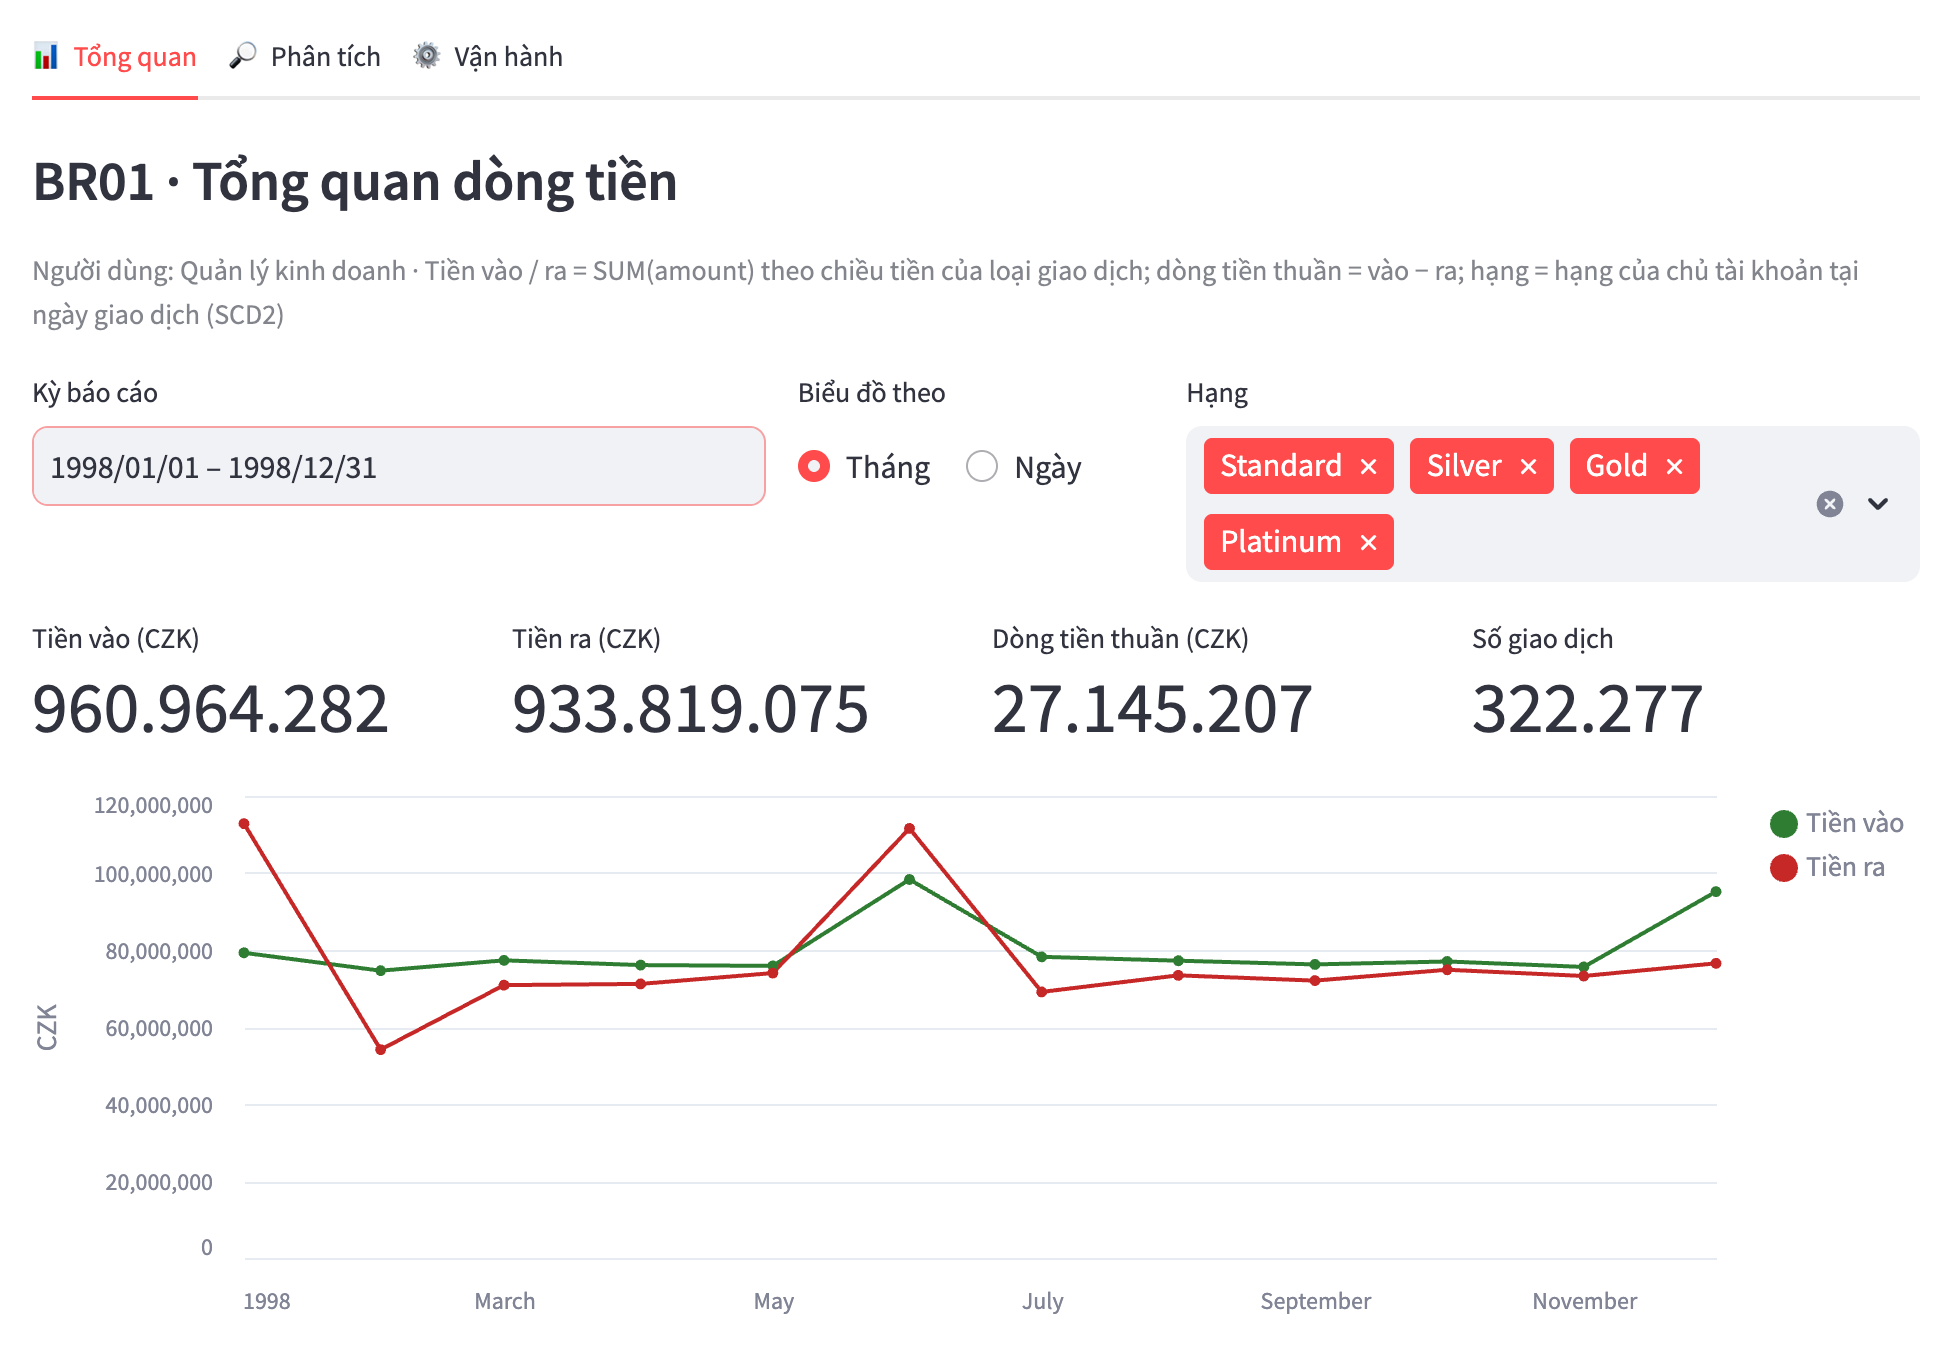
\includegraphics[width=\columnwidth]{app_overview}
\caption{Overview tab (U01, BR01): cash-flow KPIs and the monthly chart for 1998.}
\label{fig:app-overview}
\end{figure}

\begin{figure}[!t]
\centering
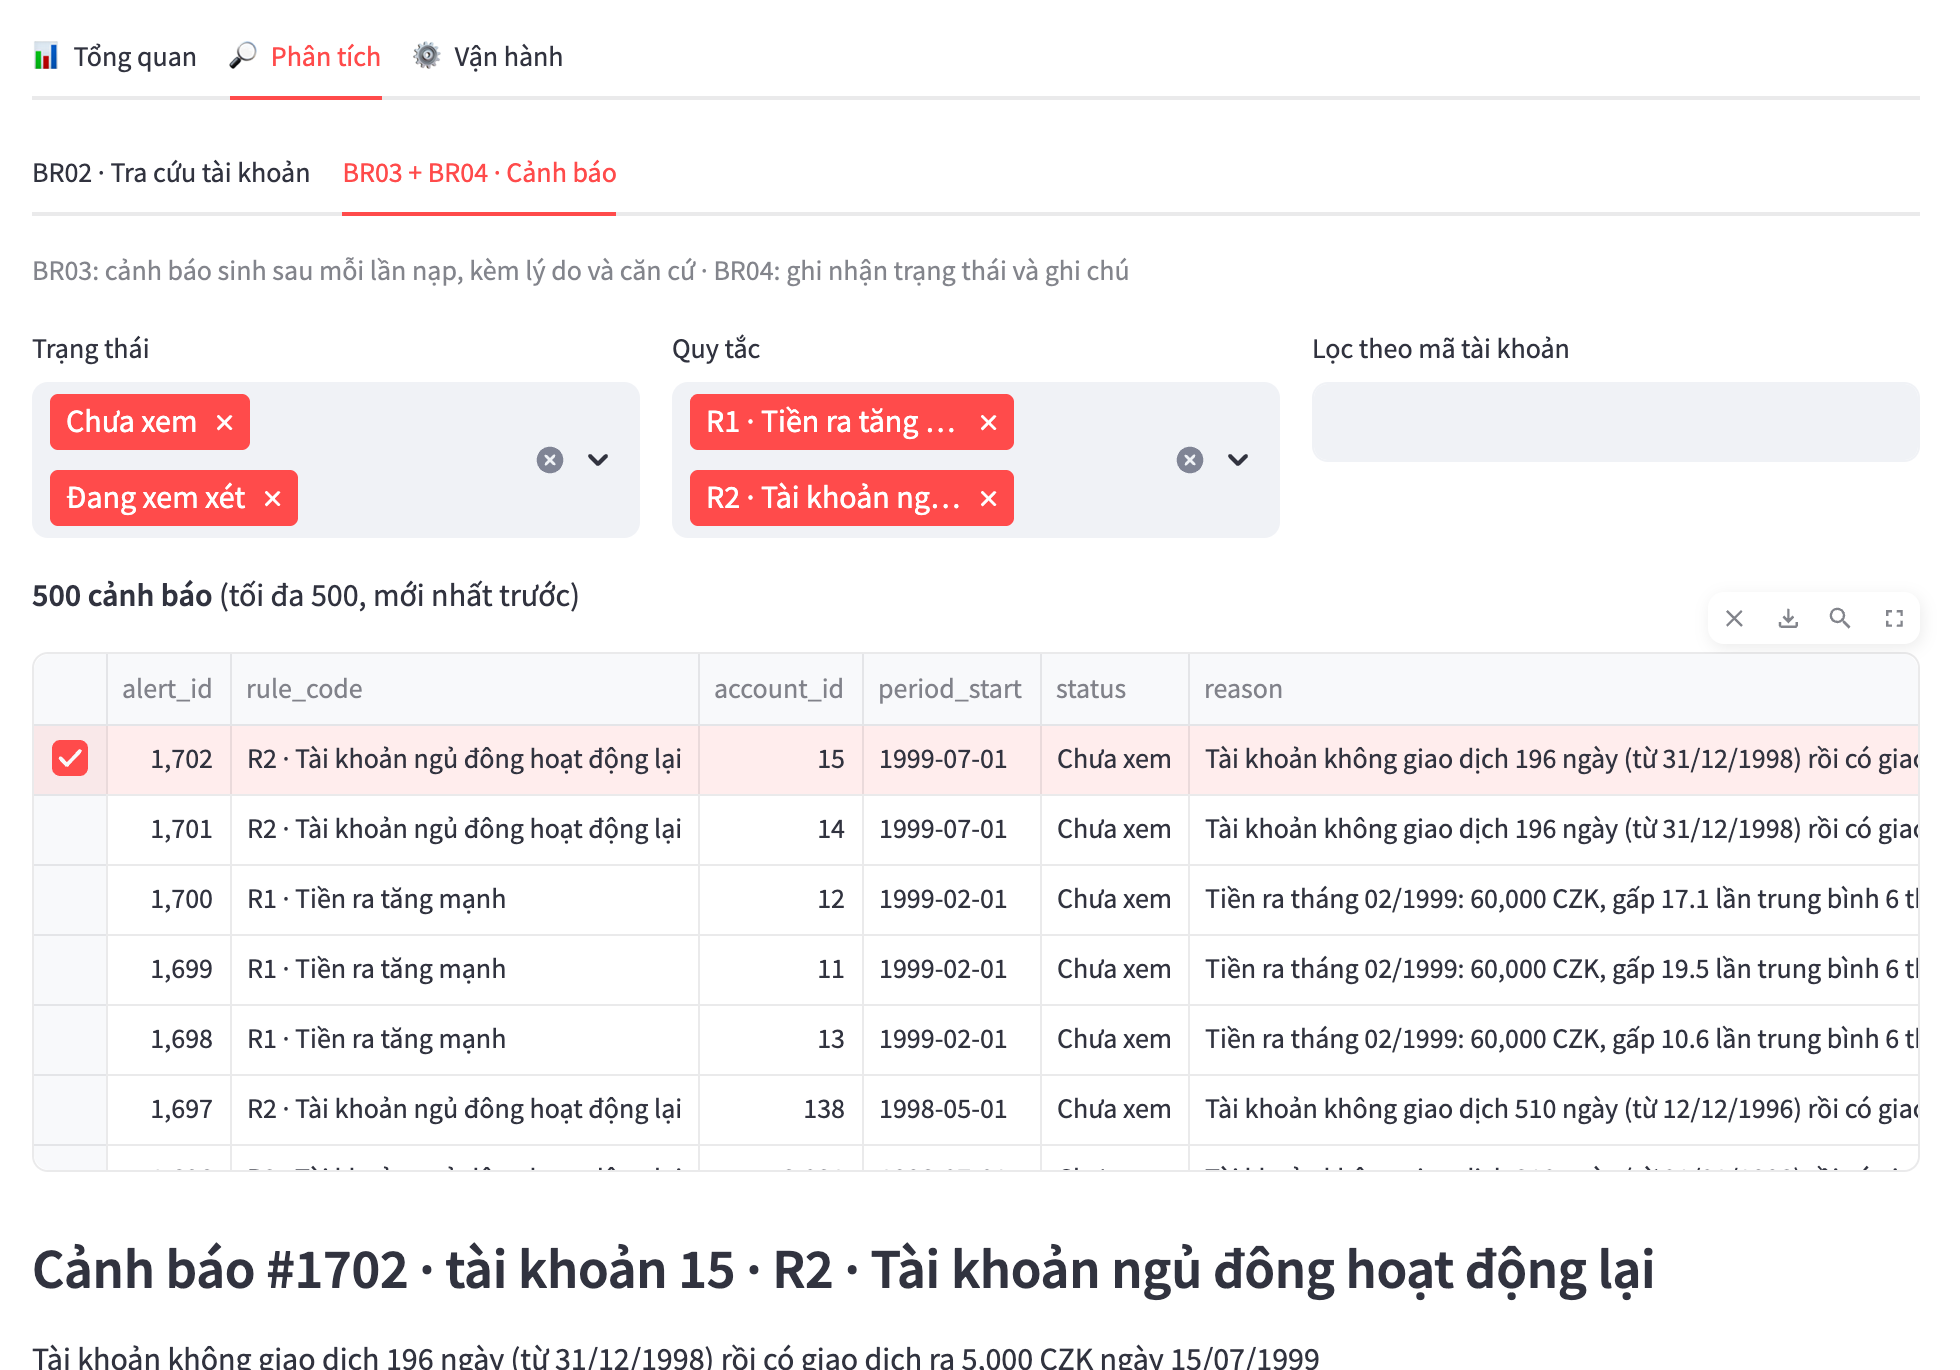
\includegraphics[width=\columnwidth]{app_alert}
\caption{Analysis tab (U02, BR03): alert list with rule, account, period, status, and reason.}
\label{fig:app-alert}
\end{figure}

\subsection{Interpretation}
The results suggest that the proposed solution meets the three criteria. The warehouse
reproduces the source exactly, and isolation of defective records, idempotent re-runs,
alerts without duplicates, restore, and history preservation behaved as specified. The column
store appears to be the right choice for the aggregations that define the warehouse
workload, with an advantage that grows with the data. The two alternatives are each better at
one thing---PostgreSQL at point lookups and single-row updates, the One Big Table at join-free
scans---and the architecture uses the first where it matters: the operational store.

\subsection{Threats to Validity}
All systems shared one virtual machine with the client, and PostgreSQL had moderate settings;
partitioning or materialized views could narrow its gap. ``Cold'' runs are only partly cold,
since the page cache of the operating system could not be dropped. The $\times$10 data is a
replica and may compress better than real data. The tier and the scenarios are simulated, and
the interactions were measured by a script, not with real users.


%% =====================================================================
\section{Conclusions and Recommendations}
\label{sec:conclusion}

The Kimball warehouse on ClickHouse, fed by a controlled batch pipeline and paired with a
PostgreSQL operational store, met all three criteria. On \emph{data correctness}, all eight
scenarios passed and cash-flow figures equal the source to the cent, with history preserved
across tier changes. On \emph{performance}, ClickHouse answered aggregations 3.3--22 times
faster than PostgreSQL (7--28 times at $\times$10) in 8.7 times less space, the star schema
avoided correction costs of up to 1.5 million rows, and the operational store was 8--70 times
faster and safer in PostgreSQL. On \emph{effectiveness}, every BR was answered in one to three
interactions within half a second.

\textbf{Recommendations.} Use a column store for the warehouse, whose users mainly aggregate,
and a relational database for the operational data, which is updated in place and must
enforce constraints. Filter the fact table on its own key first in lookups.

\textbf{Limitations and future work.} The data ends in 1998 and the tier is simulated;
end-of-period balances and access control are missing. Future work: access control per user
group, further business processes such as loans, measurements at larger scale and on a
cluster, and learned anomaly detection evaluated on the same scenarios.


%% =====================================================================
\appendices

\section{Reproducibility}
\label{App:Reproducibility}
Code and scripts: \url{https://github.com/quanndc/data-engineer-bank-project}.
\texttt{make up}, \texttt{make schema}, \texttt{make load-ref}, and \texttt{make load-history}
build the warehouse; \texttt{make scenarios} and \texttt{make scenario KB=\ldots} run the
scenarios; \texttt{make evaluate} and \texttt{make bench-all} (\texttt{SCALE=10} for
$\times$10) reproduce the evaluation and the benchmarks, with results in
\texttt{docs/results/p2/}; \texttt{tools/ui\_walkthrough.py} measures the application.

\section{Work Allocation}
\label{App:Work}

\todo{Confirm the allocation with the group.}

\begin{table}[!h]
\centering
\caption{Work Allocation}
\label{tab:work}
\footnotesize
\setlength{\tabcolsep}{4pt}
\begin{tabular}{L{2.6cm} L{3.4cm} L{1.6cm}}
\toprule
\textbf{Member} & \textbf{Technical area} & \textbf{BRs} \\
\midrule
Kiet Ho Tuan Nguyen & \todo{} & \todo{} \\
Quan Minh Tran & \todo{} & \todo{} \\
Van Ngoc Huynh & \todo{} & \todo{} \\
Hai Ngoc Ho & \todo{} & \todo{} \\
\bottomrule
\end{tabular}
\end{table}


\begin{thebibliography}{99}

\bibitem{berka1999}
P.~Berka, ``Guide to the financial data set,'' in \emph{PKDD'99 Discovery Challenge},
Prague, Czech Republic, 1999. [Online]. Available:
\url{https://www.kaggle.com/datasets/marceloventura/the-berka-dataset}

\bibitem{kimball2013}
R.~Kimball and M.~Ross, \emph{The Data Warehouse Toolkit: The Definitive Guide to
Dimensional Modeling}, 3rd~ed.\hskip 1em plus 0.5em minus 0.4em\relax Indianapolis, IN,
USA: Wiley, 2013.

\bibitem{inmon2005}
W.~H. Inmon, \emph{Building the Data Warehouse}, 4th~ed.\hskip 1em plus 0.5em minus
0.4em\relax Indianapolis, IN, USA: Wiley, 2005.

\bibitem{linstedt2015}
D.~Linstedt and M.~Olschimke, \emph{Building a Scalable Data Warehouse with Data Vault
2.0}.\hskip 1em plus 0.5em minus 0.4em\relax Waltham, MA, USA: Morgan Kaufmann, 2015.

\bibitem{zaharia2016spark}
M.~Zaharia \emph{et~al.}, ``Apache Spark: A unified engine for big data processing,''
\emph{Commun. ACM}, vol.~59, no.~11, pp.~56--65, 2016.

\bibitem{schulze2024clickhouse}
R.~Schulze, T.~Schreiber, I.~Yatsishin, R.~Dahimene, and A.~Milovidov, ``ClickHouse ---
Lightning fast analytics for everyone,'' \emph{Proc. VLDB Endow.}, vol.~17, no.~12,
pp.~3731--3744, 2024.

\bibitem{stonebraker2005cstore}
M.~Stonebraker \emph{et~al.}, ``C-Store: A column-oriented DBMS,'' in \emph{Proc. VLDB},
2005, pp.~553--564.

\bibitem{abadi2008column}
D.~J. Abadi, S.~R. Madden, and N.~Hachem, ``Column-stores vs.\ row-stores: How different
are they really?'' in \emph{Proc. ACM SIGMOD}, 2008, pp.~967--980.

\bibitem{armbrust2021lakehouse}
M.~Armbrust, A.~Ghodsi, R.~Xin, and M.~Zaharia, ``Lakehouse: A new generation of open
platforms that unify data warehousing and advanced analytics,'' in \emph{Proc. CIDR}, 2021.

\bibitem{oneil2009ssb}
P.~O'Neil, E.~O'Neil, X.~Chen, and S.~Revilak, ``The Star Schema Benchmark and augmented
fact table indexing,'' in \emph{Proc. TPCTC}, LNCS vol.~5895, 2009, pp.~237--252.

\bibitem{tpch}
Transaction Processing Performance Council, ``TPC Benchmark H (Decision Support) Standard
Specification.'' [Online]. Available: \url{https://www.tpc.org/tpch/}

\bibitem{tpcds}
Transaction Processing Performance Council, ``TPC Benchmark DS Standard Specification.''
[Online]. Available: \url{https://www.tpc.org/tpcds/}

\bibitem{iso25012}
\emph{Software Engineering --- Software Product Quality Requirements and Evaluation
(SQuaRE) --- Data Quality Model}, ISO/IEC 25012:2008, 2008.

\bibitem{c4model}
S.~Brown, ``The C4 model for visualising software architecture.'' [Online]. Available:
\url{https://c4model.com}

\bibitem{streamlit}
Snowflake Inc., ``Streamlit: A faster way to build and share data apps.'' [Online].
Available: \url{https://streamlit.io}

\end{thebibliography}

\end{document}
